\documentclass[1p]{elsarticle_modified}
%\bibliographystyle{elsarticle-num}

%\usepackage[colorlinks]{hyperref}
%\usepackage{abbrmath_seonhwa} %\Abb, \Ascr, \Acal ,\Abf, \Afrak
\usepackage{amsfonts}
\usepackage{amssymb}
\usepackage{amsmath}
\usepackage{amsthm}
\usepackage{scalefnt}
\usepackage{amsbsy}
\usepackage{kotex}
\usepackage{caption}
\usepackage{subfig}
\usepackage{color}
\usepackage{graphicx}
\usepackage{xcolor} %% white, black, red, green, blue, cyan, magenta, yellow
\usepackage{float}
\usepackage{setspace}
\usepackage{hyperref}

\usepackage{tikz}
\usetikzlibrary{arrows}

\usepackage{multirow}
\usepackage{array} % fixed length table
\usepackage{hhline}

%%%%%%%%%%%%%%%%%%%%%
\makeatletter
\renewcommand*\env@matrix[1][\arraystretch]{%
	\edef\arraystretch{#1}%
	\hskip -\arraycolsep
	\let\@ifnextchar\new@ifnextchar
	\array{*\c@MaxMatrixCols c}}
\makeatother %https://tex.stackexchange.com/questions/14071/how-can-i-increase-the-line-spacing-in-a-matrix
%%%%%%%%%%%%%%%

\usepackage[normalem]{ulem}

\newcommand{\msout}[1]{\ifmmode\text{\sout{\ensuremath{#1}}}\else\sout{#1}\fi}
%SOURCE: \msout is \stkout macro in https://tex.stackexchange.com/questions/20609/strikeout-in-math-mode

\newcommand{\cancel}[1]{
	\ifmmode
	{\color{red}\msout{#1}}
	\else
	{\color{red}\sout{#1}}
	\fi
}

\newcommand{\add}[1]{
	{\color{blue}\uwave{#1}}
}

\newcommand{\replace}[2]{
	\ifmmode
	{\color{red}\msout{#1}}{\color{blue}\uwave{#2}}
	\else
	{\color{red}\sout{#1}}{\color{blue}\uwave{#2}}
	\fi
}

\newcommand{\Sol}{\mathcal{S}} %segment
\newcommand{\D}{D} %diagram
\newcommand{\A}{\mathcal{A}} %arc


%%%%%%%%%%%%%%%%%%%%%%%%%%%%%5 test

\def\sl{\operatorname{\textup{SL}}(2,\Cbb)}
\def\psl{\operatorname{\textup{PSL}}(2,\Cbb)}
\def\quan{\mkern 1mu \triangleright \mkern 1mu}

\theoremstyle{definition}
\newtheorem{thm}{Theorem}[section]
\newtheorem{prop}[thm]{Proposition}
\newtheorem{lem}[thm]{Lemma}
\newtheorem{ques}[thm]{Question}
\newtheorem{cor}[thm]{Corollary}
\newtheorem{defn}[thm]{Definition}
\newtheorem{exam}[thm]{Example}
\newtheorem{rmk}[thm]{Remark}
\newtheorem{alg}[thm]{Algorithm}

\newcommand{\I}{\sqrt{-1}}
\begin{document}

%\begin{frontmatter}
%
%\title{Boundary parabolic representations of knots up to 8 crossings}
%
%%% Group authors per affiliation:
%\author{Yunhi Cho} 
%\address{Department of Mathematics, University of Seoul, Seoul, Korea}
%\ead{yhcho@uos.ac.kr}
%
%
%\author{Seonhwa Kim} %\fnref{s_kim}}
%\address{Center for Geometry and Physics, Institute for Basic Science, Pohang, 37673, Korea}
%\ead{ryeona17@ibs.re.kr}
%
%\author{Hyuk Kim}
%\address{Department of Mathematical Sciences, Seoul National University, Seoul 08826, Korea}
%\ead{hyukkim@snu.ac.kr}
%
%\author{Seokbeom Yoon}
%\address{Department of Mathematical Sciences, Seoul National University, Seoul, 08826,  Korea}
%\ead{sbyoon15@snu.ac.kr}
%
%\begin{abstract}
%We find all boundary parabolic representation of knots up to 8 crossings.
%
%\end{abstract}
%\begin{keyword}
%    \MSC[2010] 57M25 
%\end{keyword}
%
%\end{frontmatter}

%\linenumbers
%\tableofcontents
%
\newcommand\colored[1]{\textcolor{white}{\rule[-0.35ex]{0.8em}{1.4ex}}\kern-0.8em\color{red} #1}%
%\newcommand\colored[1]{\textcolor{white}{ #1}\kern-2.17ex	\textcolor{white}{ #1}\kern-1.81ex	\textcolor{white}{ #1}\kern-2.15ex\color{red}#1	}

{\Large $\underline{12a_{0526}~(K12a_{0526})}$}

\setlength{\tabcolsep}{10pt}
\renewcommand{\arraystretch}{1.6}
\vspace{1cm}\begin{tabular}{m{100pt}>{\centering\arraybackslash}m{274pt}}
\multirow{5}{120pt}{
	\centering
	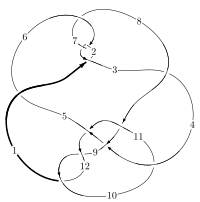
\includegraphics[width=112pt]{../../../GIT/diagram.site/Diagrams/png/1327_12a_0526.png}\\
\ \ \ A knot diagram\footnotemark}&
\allowdisplaybreaks
\textbf{Linearized knot diagam} \\
\cline{2-2}
 &
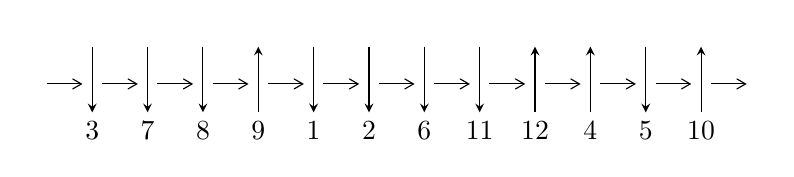
\begin{tikzpicture}[x=20pt, y=17pt]
	% nodes
	\node (C0) at (0, 0) {};
	\node (C1) at (1, 0) {};
	\node (C1U) at (1, +1) {};
	\node (C1D) at (1, -1) {3};

	\node (C2) at (2, 0) {};
	\node (C2U) at (2, +1) {};
	\node (C2D) at (2, -1) {7};

	\node (C3) at (3, 0) {};
	\node (C3U) at (3, +1) {};
	\node (C3D) at (3, -1) {8};

	\node (C4) at (4, 0) {};
	\node (C4U) at (4, +1) {};
	\node (C4D) at (4, -1) {9};

	\node (C5) at (5, 0) {};
	\node (C5U) at (5, +1) {};
	\node (C5D) at (5, -1) {1};

	\node (C6) at (6, 0) {};
	\node (C6U) at (6, +1) {};
	\node (C6D) at (6, -1) {2};

	\node (C7) at (7, 0) {};
	\node (C7U) at (7, +1) {};
	\node (C7D) at (7, -1) {6};

	\node (C8) at (8, 0) {};
	\node (C8U) at (8, +1) {};
	\node (C8D) at (8, -1) {11};

	\node (C9) at (9, 0) {};
	\node (C9U) at (9, +1) {};
	\node (C9D) at (9, -1) {12};

	\node (C10) at (10, 0) {};
	\node (C10U) at (10, +1) {};
	\node (C10D) at (10, -1) {4};

	\node (C11) at (11, 0) {};
	\node (C11U) at (11, +1) {};
	\node (C11D) at (11, -1) {5};

	\node (C12) at (12, 0) {};
	\node (C12U) at (12, +1) {};
	\node (C12D) at (12, -1) {10};
	\node (C13) at (13, 0) {};

	% arrows
	\draw[->,>={angle 60}]
	(C0) edge (C1) (C1) edge (C2) (C2) edge (C3) (C3) edge (C4) (C4) edge (C5) (C5) edge (C6) (C6) edge (C7) (C7) edge (C8) (C8) edge (C9) (C9) edge (C10) (C10) edge (C11) (C11) edge (C12) (C12) edge (C13) ;	\draw[->,>=stealth]
	(C1U) edge (C1D) (C2U) edge (C2D) (C3U) edge (C3D) (C4D) edge (C4U) (C5U) edge (C5D) (C6U) edge (C6D) (C7U) edge (C7D) (C8U) edge (C8D) (C9D) edge (C9U) (C10D) edge (C10U) (C11U) edge (C11D) (C12D) edge (C12U) ;
	\end{tikzpicture} \\
\hhline{~~} \\& 
\textbf{Solving Sequence} \\ \cline{2-2} 
 &
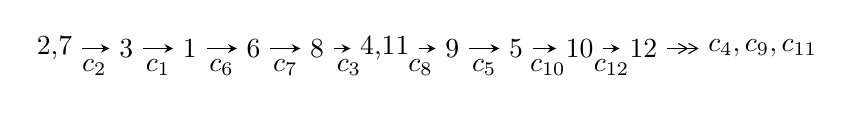
\begin{tikzpicture}[x=23pt, y=7pt]
	% node
	\node (A0) at (-1/8, 0) {2,7};
	\node (A1) at (1, 0) {3};
	\node (A2) at (2, 0) {1};
	\node (A3) at (3, 0) {6};
	\node (A4) at (4, 0) {8};
	\node (A5) at (81/16, 0) {4,11};
	\node (A6) at (49/8, 0) {9};
	\node (A7) at (57/8, 0) {5};
	\node (A8) at (65/8, 0) {10};
	\node (A9) at (73/8, 0) {12};
	\node (C1) at (1/2, -1) {$c_{2}$};
	\node (C2) at (3/2, -1) {$c_{1}$};
	\node (C3) at (5/2, -1) {$c_{6}$};
	\node (C4) at (7/2, -1) {$c_{7}$};
	\node (C5) at (9/2, -1) {$c_{3}$};
	\node (C6) at (45/8, -1) {$c_{8}$};
	\node (C7) at (53/8, -1) {$c_{5}$};
	\node (C8) at (61/8, -1) {$c_{10}$};
	\node (C9) at (69/8, -1) {$c_{12}$};
	\node (A10) at (11, 0) {$c_{4},c_{9},c_{11}$};

	% edge
	\draw[->,>=stealth]	
	(A0) edge (A1) (A1) edge (A2) (A2) edge (A3) (A3) edge (A4) (A4) edge (A5) (A5) edge (A6) (A6) edge (A7) (A7) edge (A8) (A8) edge (A9) ;
	\draw[->>,>={angle 60}]	
	(A9) edge (A10);
\end{tikzpicture} \\ 

\end{tabular} \\

\footnotetext{
The image of knot diagram is generated by the software ``\textbf{Draw programme}" developed by Andrew Bartholomew(\url{http://www.layer8.co.uk/maths/draw/index.htm\#Running-draw}), where we modified some parts for our purpose(\url{https://github.com/CATsTAILs/LinksPainter}).
}\phantom \\ \newline 
\centering \textbf{Ideals for irreducible components\footnotemark of $X_{\text{par}}$} 
 
\begin{align*}
I^u_{1}&=\langle 
1.43587\times10^{35} u^{107}+2.94893\times10^{35} u^{106}+\cdots+6.98068\times10^{34} b+3.66969\times10^{35},\\
\phantom{I^u_{1}}&\phantom{= \langle  }3.25085\times10^{35} u^{107}+4.64698\times10^{35} u^{106}+\cdots+6.98068\times10^{34} a+7.03973\times10^{34},\;u^{108}+2 u^{107}+\cdots+3 u+1\rangle \\
I^u_{2}&=\langle 
b+1,\;- u^2+a- u,\;u^3+u^2-1\rangle \\
\\
\end{align*}
\raggedright * 2 irreducible components of $\dim_{\mathbb{C}}=0$, with total 111 representations.\\
\footnotetext{All coefficients of polynomials are rational numbers. But the coefficients are sometimes approximated in decimal forms when there is not enough margin.}
\newpage
\renewcommand{\arraystretch}{1}
\centering \section*{I. $I^u_{1}= \langle 1.44\times10^{35} u^{107}+2.95\times10^{35} u^{106}+\cdots+6.98\times10^{34} b+3.67\times10^{35},\;3.25\times10^{35} u^{107}+4.65\times10^{35} u^{106}+\cdots+6.98\times10^{34} a+7.04\times10^{34},\;u^{108}+2 u^{107}+\cdots+3 u+1 \rangle$}
\flushleft \textbf{(i) Arc colorings}\\
\begin{tabular}{m{7pt} m{180pt} m{7pt} m{180pt} }
\flushright $a_{2}=$&$\begin{pmatrix}1\\0\end{pmatrix}$ \\
\flushright $a_{7}=$&$\begin{pmatrix}0\\u\end{pmatrix}$ \\
\flushright $a_{3}=$&$\begin{pmatrix}1\\u^2\end{pmatrix}$ \\
\flushright $a_{1}=$&$\begin{pmatrix}- u^2+1\\- u^4\end{pmatrix}$ \\
\flushright $a_{6}=$&$\begin{pmatrix}u\\u\end{pmatrix}$ \\
\flushright $a_{8}=$&$\begin{pmatrix}- u^3\\- u^3+u\end{pmatrix}$ \\
\flushright $a_{4}=$&$\begin{pmatrix}- u^8+u^6- u^4+1\\- u^8+2 u^6-2 u^4+2 u^2\end{pmatrix}$ \\
\flushright $a_{11}=$&$\begin{pmatrix}-4.65692 u^{107}-6.65692 u^{106}+\cdots-6.39711 u-1.00846\\-2.05692 u^{107}-4.22441 u^{106}+\cdots-16.7623 u-5.25692\end{pmatrix}$ \\
\flushright $a_{9}=$&$\begin{pmatrix}0.622547 u^{107}+1.02255 u^{106}+\cdots-3.55169 u+0.111274\\0.222547 u^{107}-0.380109 u^{106}+\cdots+1.75637 u+0.622547\end{pmatrix}$ \\
\flushright $a_{5}=$&$\begin{pmatrix}- u^7+2 u^5-2 u^3+2 u\\- u^9+u^7- u^5+u\end{pmatrix}$ \\
\flushright $a_{10}=$&$\begin{pmatrix}-5.78807 u^{107}-9.58807 u^{106}+\cdots+0.732755 u-0.554037\\-3.18807 u^{107}-5.54842 u^{106}+\cdots-14.3702 u-4.78807\end{pmatrix}$ \\
\flushright $a_{12}=$&$\begin{pmatrix}-5.68213 u^{107}-9.28213 u^{106}+\cdots-0.971272 u-0.00106654\\-3.28213 u^{107}-5.84102 u^{106}+\cdots-14.0053 u-4.68213\end{pmatrix}$\\&\end{tabular}
\flushleft \textbf{(ii) Obstruction class $= -1$}\\~\\
\flushleft \textbf{(iii) Cusp Shapes $= -3.18066 u^{107}-12.3213 u^{106}+\cdots-15.7876 u-9.30066$}\\~\\
\newpage\renewcommand{\arraystretch}{1}
\flushleft \textbf{(iv) u-Polynomials at the component}\newline \\
\begin{tabular}{m{50pt}|m{274pt}}
Crossings & \hspace{64pt}u-Polynomials at each crossing \\
\hline $$\begin{aligned}c_{1},c_{7}\end{aligned}$$&$\begin{aligned}
&u^{108}+38 u^{107}+\cdots+7 u+1
\end{aligned}$\\
\hline $$\begin{aligned}c_{2},c_{6}\end{aligned}$$&$\begin{aligned}
&u^{108}-2 u^{107}+\cdots-3 u+1
\end{aligned}$\\
\hline $$\begin{aligned}c_{3},c_{5}\end{aligned}$$&$\begin{aligned}
&u^{108}+2 u^{107}+\cdots+9913 u+8017
\end{aligned}$\\
\hline $$\begin{aligned}c_{4}\end{aligned}$$&$\begin{aligned}
&u^{108}-2 u^{107}+\cdots+u-1
\end{aligned}$\\
\hline $$\begin{aligned}c_{8}\end{aligned}$$&$\begin{aligned}
&u^{108}-17 u^{107}+\cdots-20 u+8
\end{aligned}$\\
\hline $$\begin{aligned}c_{9},c_{12}\end{aligned}$$&$\begin{aligned}
&u^{108}+4 u^{107}+\cdots-28 u-1
\end{aligned}$\\
\hline $$\begin{aligned}c_{10}\end{aligned}$$&$\begin{aligned}
&u^{108}+3 u^{107}+\cdots+1284 u+109
\end{aligned}$\\
\hline $$\begin{aligned}c_{11}\end{aligned}$$&$\begin{aligned}
&u^{108}+u^{107}+\cdots+54 u+1
\end{aligned}$\\
\hline
\end{tabular}\\~\\
\newpage\renewcommand{\arraystretch}{1}
\flushleft \textbf{(v) Riley Polynomials at the component}\newline \\
\begin{tabular}{m{50pt}|m{274pt}}
Crossings & \hspace{64pt}Riley Polynomials at each crossing \\
\hline $$\begin{aligned}c_{1},c_{7}\end{aligned}$$&$\begin{aligned}
&y^{108}+66 y^{107}+\cdots+49 y+1
\end{aligned}$\\
\hline $$\begin{aligned}c_{2},c_{6}\end{aligned}$$&$\begin{aligned}
&y^{108}-38 y^{107}+\cdots-7 y+1
\end{aligned}$\\
\hline $$\begin{aligned}c_{3},c_{5}\end{aligned}$$&$\begin{aligned}
&y^{108}-78 y^{107}+\cdots-1545833123 y+64272289
\end{aligned}$\\
\hline $$\begin{aligned}c_{4}\end{aligned}$$&$\begin{aligned}
&y^{108}-14 y^{107}+\cdots-7 y+1
\end{aligned}$\\
\hline $$\begin{aligned}c_{8}\end{aligned}$$&$\begin{aligned}
&y^{108}-21 y^{107}+\cdots-2256 y+64
\end{aligned}$\\
\hline $$\begin{aligned}c_{9},c_{12}\end{aligned}$$&$\begin{aligned}
&y^{108}-64 y^{107}+\cdots-780 y+1
\end{aligned}$\\
\hline $$\begin{aligned}c_{10}\end{aligned}$$&$\begin{aligned}
&y^{108}+105 y^{107}+\cdots+224182 y+11881
\end{aligned}$\\
\hline $$\begin{aligned}c_{11}\end{aligned}$$&$\begin{aligned}
&y^{108}+97 y^{107}+\cdots-3282 y+1
\end{aligned}$\\
\hline
\end{tabular}\\~\\
\newpage\flushleft \textbf{(vi) Complex Volumes and Cusp Shapes}
$$\begin{array}{c|c|c}  
\text{Solutions to }I^u_{1}& \I (\text{vol} + \sqrt{-1}CS) & \text{Cusp shape}\\
 \hline 
\begin{aligned}
u &= -0.597771 + 0.813650 I \\
a &= \phantom{-}2.47839 + 0.85182 I \\
b &= \phantom{-}2.57699 - 1.74065 I\end{aligned}
 & \phantom{-}0.91550 - 12.81660 I & \phantom{-0.000000 } 0 \\ \hline\begin{aligned}
u &= -0.597771 - 0.813650 I \\
a &= \phantom{-}2.47839 - 0.85182 I \\
b &= \phantom{-}2.57699 + 1.74065 I\end{aligned}
 & \phantom{-}0.91550 + 12.81660 I & \phantom{-0.000000 } 0 \\ \hline\begin{aligned}
u &= -0.586515 + 0.785999 I \\
a &= -2.58131 - 1.17591 I \\
b &= -2.78106 + 1.56187 I\end{aligned}
 & -2.76135 - 6.51854 I & \phantom{-0.000000 } 0 \\ \hline\begin{aligned}
u &= -0.586515 - 0.785999 I \\
a &= -2.58131 + 1.17591 I \\
b &= -2.78106 - 1.56187 I\end{aligned}
 & -2.76135 + 6.51854 I & \phantom{-0.000000 } 0 \\ \hline\begin{aligned}
u &= \phantom{-}0.614242 + 0.813810 I \\
a &= \phantom{-}1.370720 - 0.107661 I \\
b &= \phantom{-}0.98107 + 1.24217 I\end{aligned}
 & -0.36628 + 4.95266 I & \phantom{-0.000000 } 0 \\ \hline\begin{aligned}
u &= \phantom{-}0.614242 - 0.813810 I \\
a &= \phantom{-}1.370720 + 0.107661 I \\
b &= \phantom{-}0.98107 - 1.24217 I\end{aligned}
 & -0.36628 - 4.95266 I & \phantom{-0.000000 } 0 \\ \hline\begin{aligned}
u &= \phantom{-}0.993276 + 0.256239 I \\
a &= \phantom{-}0.048345 + 0.497832 I \\
b &= -0.417849 + 0.962950 I\end{aligned}
 & -0.21980 + 2.28779 I & \phantom{-0.000000 } 0 \\ \hline\begin{aligned}
u &= \phantom{-}0.993276 - 0.256239 I \\
a &= \phantom{-}0.048345 - 0.497832 I \\
b &= -0.417849 - 0.962950 I\end{aligned}
 & -0.21980 - 2.28779 I & \phantom{-0.000000 } 0 \\ \hline\begin{aligned}
u &= -0.607429 + 0.758889 I \\
a &= \phantom{-}1.10687 - 1.94850 I \\
b &= -0.65726 - 1.68774 I\end{aligned}
 & \phantom{-}2.45525 - 4.40691 I & \phantom{-0.000000 } 0 \\ \hline\begin{aligned}
u &= -0.607429 - 0.758889 I \\
a &= \phantom{-}1.10687 + 1.94850 I \\
b &= -0.65726 + 1.68774 I\end{aligned}
 & \phantom{-}2.45525 + 4.40691 I & \phantom{-0.000000 } 0\\
 \hline 
 \end{array}$$\newpage$$\begin{array}{c|c|c}  
\text{Solutions to }I^u_{1}& \I (\text{vol} + \sqrt{-1}CS) & \text{Cusp shape}\\
 \hline 
\begin{aligned}
u &= -0.967017 + 0.354553 I \\
a &= \phantom{-}0.685909 + 0.472926 I \\
b &= \phantom{-}1.49049 + 0.16949 I\end{aligned}
 & \phantom{-}0.30361 + 8.27780 I & \phantom{-0.000000 } 0 \\ \hline\begin{aligned}
u &= -0.967017 - 0.354553 I \\
a &= \phantom{-}0.685909 - 0.472926 I \\
b &= \phantom{-}1.49049 - 0.16949 I\end{aligned}
 & \phantom{-}0.30361 - 8.27780 I & \phantom{-0.000000 } 0 \\ \hline\begin{aligned}
u &= \phantom{-}0.557597 + 0.778279 I \\
a &= -1.43951 + 0.23035 I \\
b &= -1.35512 - 1.16412 I\end{aligned}
 & -2.06069 + 1.57945 I & \phantom{-0.000000 } 0 \\ \hline\begin{aligned}
u &= \phantom{-}0.557597 - 0.778279 I \\
a &= -1.43951 - 0.23035 I \\
b &= -1.35512 + 1.16412 I\end{aligned}
 & -2.06069 - 1.57945 I & \phantom{-0.000000 } 0 \\ \hline\begin{aligned}
u &= \phantom{-}0.862517 + 0.409462 I \\
a &= \phantom{-}0.385572 - 0.577994 I \\
b &= \phantom{-}0.641697 - 0.857621 I\end{aligned}
 & -1.97653 - 1.26355 I & \phantom{-0.000000 } 0 \\ \hline\begin{aligned}
u &= \phantom{-}0.862517 - 0.409462 I \\
a &= \phantom{-}0.385572 + 0.577994 I \\
b &= \phantom{-}0.641697 + 0.857621 I\end{aligned}
 & -1.97653 + 1.26355 I & \phantom{-0.000000 } 0 \\ \hline\begin{aligned}
u &= -0.625012 + 0.720883 I \\
a &= \phantom{-}3.20428 + 0.82917 I \\
b &= \phantom{-}2.95448 - 1.87384 I\end{aligned}
 & \phantom{-}3.68605 - 0.74056 I & \phantom{-0.000000 } 0 \\ \hline\begin{aligned}
u &= -0.625012 - 0.720883 I \\
a &= \phantom{-}3.20428 - 0.82917 I \\
b &= \phantom{-}2.95448 + 1.87384 I\end{aligned}
 & \phantom{-}3.68605 + 0.74056 I & \phantom{-0.000000 } 0 \\ \hline\begin{aligned}
u &= \phantom{-}0.588671 + 0.741137 I \\
a &= \phantom{-}0.539890 - 1.301750 I \\
b &= \phantom{-}1.94501 - 1.70423 I\end{aligned}
 & \phantom{-}0.76621 + 1.69194 I & \phantom{-0.000000 } 0 \\ \hline\begin{aligned}
u &= \phantom{-}0.588671 - 0.741137 I \\
a &= \phantom{-}0.539890 + 1.301750 I \\
b &= \phantom{-}1.94501 + 1.70423 I\end{aligned}
 & \phantom{-}0.76621 - 1.69194 I & \phantom{-0.000000 } 0\\
 \hline 
 \end{array}$$\newpage$$\begin{array}{c|c|c}  
\text{Solutions to }I^u_{1}& \I (\text{vol} + \sqrt{-1}CS) & \text{Cusp shape}\\
 \hline 
\begin{aligned}
u &= -0.815039 + 0.672331 I \\
a &= \phantom{-}1.30528 + 1.09070 I \\
b &= \phantom{-}1.63606 - 0.42604 I\end{aligned}
 & \phantom{-}2.61814 + 2.06099 I & \phantom{-0.000000 } 0 \\ \hline\begin{aligned}
u &= -0.815039 - 0.672331 I \\
a &= \phantom{-}1.30528 - 1.09070 I \\
b &= \phantom{-}1.63606 + 0.42604 I\end{aligned}
 & \phantom{-}2.61814 - 2.06099 I & \phantom{-0.000000 } 0 \\ \hline\begin{aligned}
u &= \phantom{-}0.791206 + 0.707863 I \\
a &= \phantom{-}1.242420 - 0.296906 I \\
b &= \phantom{-}0.289663 + 0.875878 I\end{aligned}
 & \phantom{-}2.57323 + 1.47652 I & \phantom{-0.000000 } 0 \\ \hline\begin{aligned}
u &= \phantom{-}0.791206 - 0.707863 I \\
a &= \phantom{-}1.242420 + 0.296906 I \\
b &= \phantom{-}0.289663 - 0.875878 I\end{aligned}
 & \phantom{-}2.57323 - 1.47652 I & \phantom{-0.000000 } 0 \\ \hline\begin{aligned}
u &= \phantom{-}1.06533\phantom{ +0.000000I} \\
a &= \phantom{-}1.87148\phantom{ +0.000000I} \\
b &= -1.09473\phantom{ +0.000000I}\end{aligned}
 & -1.61062\phantom{ +0.000000I} & \phantom{-0.000000 } 0 \\ \hline\begin{aligned}
u &= \phantom{-}1.083580 + 0.029651 I \\
a &= \phantom{-}0.428417 - 0.305662 I \\
b &= -0.275728 + 1.238730 I\end{aligned}
 & -3.22980 - 3.58406 I & \phantom{-0.000000 } 0 \\ \hline\begin{aligned}
u &= \phantom{-}1.083580 - 0.029651 I \\
a &= \phantom{-}0.428417 + 0.305662 I \\
b &= -0.275728 - 1.238730 I\end{aligned}
 & -3.22980 + 3.58406 I & \phantom{-0.000000 } 0 \\ \hline\begin{aligned}
u &= -1.091440 + 0.011709 I \\
a &= \phantom{-}0.73071 - 2.26932 I \\
b &= -0.154395 - 0.804597 I\end{aligned}
 & -4.77450 + 0.69884 I & \phantom{-0.000000 } 0 \\ \hline\begin{aligned}
u &= -1.091440 - 0.011709 I \\
a &= \phantom{-}0.73071 + 2.26932 I \\
b &= -0.154395 + 0.804597 I\end{aligned}
 & -4.77450 - 0.69884 I & \phantom{-0.000000 } 0 \\ \hline\begin{aligned}
u &= -0.856102 + 0.680324 I \\
a &= -3.16956 - 4.60118 I \\
b &= -6.17544 - 1.38034 I\end{aligned}
 & \phantom{-}4.07616 + 2.62315 I & \phantom{-0.000000 } 0\\
 \hline 
 \end{array}$$\newpage$$\begin{array}{c|c|c}  
\text{Solutions to }I^u_{1}& \I (\text{vol} + \sqrt{-1}CS) & \text{Cusp shape}\\
 \hline 
\begin{aligned}
u &= -0.856102 - 0.680324 I \\
a &= -3.16956 + 4.60118 I \\
b &= -6.17544 + 1.38034 I\end{aligned}
 & \phantom{-}4.07616 - 2.62315 I & \phantom{-0.000000 } 0 \\ \hline\begin{aligned}
u &= -0.757826 + 0.790886 I \\
a &= \phantom{-}0.186346 - 0.810336 I \\
b &= -0.453992 - 0.337006 I\end{aligned}
 & \phantom{-}6.40107 + 3.53173 I & \phantom{-0.000000 } 0 \\ \hline\begin{aligned}
u &= -0.757826 - 0.790886 I \\
a &= \phantom{-}0.186346 + 0.810336 I \\
b &= -0.453992 + 0.337006 I\end{aligned}
 & \phantom{-}6.40107 - 3.53173 I & \phantom{-0.000000 } 0 \\ \hline\begin{aligned}
u &= \phantom{-}0.491909 + 0.756563 I \\
a &= -1.250010 + 0.380217 I \\
b &= -1.251750 - 0.642698 I\end{aligned}
 & -2.40500 + 1.31068 I & \phantom{-0.000000 } 0 \\ \hline\begin{aligned}
u &= \phantom{-}0.491909 - 0.756563 I \\
a &= -1.250010 - 0.380217 I \\
b &= -1.251750 + 0.642698 I\end{aligned}
 & -2.40500 - 1.31068 I & \phantom{-0.000000 } 0 \\ \hline\begin{aligned}
u &= \phantom{-}0.568811 + 0.700498 I \\
a &= \phantom{-}0.923748 + 0.518614 I \\
b &= -0.06859 + 2.30340 I\end{aligned}
 & \phantom{-}0.504377 + 0.446786 I & \phantom{-0.000000 } 0 \\ \hline\begin{aligned}
u &= \phantom{-}0.568811 - 0.700498 I \\
a &= \phantom{-}0.923748 - 0.518614 I \\
b &= -0.06859 - 2.30340 I\end{aligned}
 & \phantom{-}0.504377 - 0.446786 I & \phantom{-0.000000 } 0 \\ \hline\begin{aligned}
u &= \phantom{-}0.840437 + 0.708054 I \\
a &= -0.153381 + 0.428703 I \\
b &= -0.65198 + 1.39073 I\end{aligned}
 & \phantom{-}6.23476 - 0.88816 I & \phantom{-0.000000 } 0 \\ \hline\begin{aligned}
u &= \phantom{-}0.840437 - 0.708054 I \\
a &= -0.153381 - 0.428703 I \\
b &= -0.65198 - 1.39073 I\end{aligned}
 & \phantom{-}6.23476 + 0.88816 I & \phantom{-0.000000 } 0 \\ \hline\begin{aligned}
u &= -0.854464 + 0.254519 I \\
a &= -1.106020 + 0.127999 I \\
b &= -1.49389 + 0.29078 I\end{aligned}
 & -2.63759 + 3.47259 I & \phantom{-0.000000 } 0\\
 \hline 
 \end{array}$$\newpage$$\begin{array}{c|c|c}  
\text{Solutions to }I^u_{1}& \I (\text{vol} + \sqrt{-1}CS) & \text{Cusp shape}\\
 \hline 
\begin{aligned}
u &= -0.854464 - 0.254519 I \\
a &= -1.106020 - 0.127999 I \\
b &= -1.49389 - 0.29078 I\end{aligned}
 & -2.63759 - 3.47259 I & \phantom{-0.000000 } 0 \\ \hline\begin{aligned}
u &= \phantom{-}0.794482 + 0.774864 I \\
a &= -1.360950 + 0.258430 I \\
b &= -0.607855 - 0.855698 I\end{aligned}
 & \phantom{-}7.00651 + 6.05760 I & \phantom{-0.000000 } 0 \\ \hline\begin{aligned}
u &= \phantom{-}0.794482 - 0.774864 I \\
a &= -1.360950 - 0.258430 I \\
b &= -0.607855 + 0.855698 I\end{aligned}
 & \phantom{-}7.00651 - 6.05760 I & \phantom{-0.000000 } 0 \\ \hline\begin{aligned}
u &= -0.888479 + 0.670392 I \\
a &= -0.101572 + 1.357190 I \\
b &= \phantom{-}1.25584 + 1.33718 I\end{aligned}
 & \phantom{-}2.39366 + 3.13373 I & \phantom{-0.000000 } 0 \\ \hline\begin{aligned}
u &= -0.888479 - 0.670392 I \\
a &= -0.101572 - 1.357190 I \\
b &= \phantom{-}1.25584 - 1.33718 I\end{aligned}
 & \phantom{-}2.39366 - 3.13373 I & \phantom{-0.000000 } 0 \\ \hline\begin{aligned}
u &= \phantom{-}1.112990 + 0.038874 I \\
a &= -1.58654 + 0.00313 I \\
b &= \phantom{-}0.786207 + 0.474131 I\end{aligned}
 & -8.68488 - 5.47508 I & \phantom{-0.000000 } 0 \\ \hline\begin{aligned}
u &= \phantom{-}1.112990 - 0.038874 I \\
a &= -1.58654 - 0.00313 I \\
b &= \phantom{-}0.786207 - 0.474131 I\end{aligned}
 & -8.68488 + 5.47508 I & \phantom{-0.000000 } 0 \\ \hline\begin{aligned}
u &= -1.111610 + 0.073871 I \\
a &= \phantom{-}0.639895 + 0.430578 I \\
b &= -0.517929 + 0.148112 I\end{aligned}
 & -6.60406 + 4.11832 I & \phantom{-0.000000 } 0 \\ \hline\begin{aligned}
u &= -1.111610 - 0.073871 I \\
a &= \phantom{-}0.639895 - 0.430578 I \\
b &= -0.517929 - 0.148112 I\end{aligned}
 & -6.60406 - 4.11832 I & \phantom{-0.000000 } 0 \\ \hline\begin{aligned}
u &= \phantom{-}0.872592 + 0.704880 I \\
a &= -1.305510 + 0.486497 I \\
b &= -0.426934 - 0.224892 I\end{aligned}
 & \phantom{-}6.13711 - 4.51816 I & \phantom{-0.000000 } 0\\
 \hline 
 \end{array}$$\newpage$$\begin{array}{c|c|c}  
\text{Solutions to }I^u_{1}& \I (\text{vol} + \sqrt{-1}CS) & \text{Cusp shape}\\
 \hline 
\begin{aligned}
u &= \phantom{-}0.872592 - 0.704880 I \\
a &= -1.305510 - 0.486497 I \\
b &= -0.426934 + 0.224892 I\end{aligned}
 & \phantom{-}6.13711 + 4.51816 I & \phantom{-0.000000 } 0 \\ \hline\begin{aligned}
u &= \phantom{-}1.124510 + 0.063645 I \\
a &= \phantom{-}1.57274 - 0.13635 I \\
b &= -0.613678 - 0.384341 I\end{aligned}
 & -5.29137 - 11.81510 I & \phantom{-0.000000 } 0 \\ \hline\begin{aligned}
u &= \phantom{-}1.124510 - 0.063645 I \\
a &= \phantom{-}1.57274 + 0.13635 I \\
b &= -0.613678 + 0.384341 I\end{aligned}
 & -5.29137 + 11.81510 I & \phantom{-0.000000 } 0 \\ \hline\begin{aligned}
u &= -1.126880 + 0.022051 I \\
a &= -1.110330 - 0.281031 I \\
b &= \phantom{-}0.323711 - 0.092251 I\end{aligned}
 & -7.89299 + 0.30667 I & \phantom{-0.000000 } 0 \\ \hline\begin{aligned}
u &= -1.126880 - 0.022051 I \\
a &= -1.110330 + 0.281031 I \\
b &= \phantom{-}0.323711 + 0.092251 I\end{aligned}
 & -7.89299 - 0.30667 I & \phantom{-0.000000 } 0 \\ \hline\begin{aligned}
u &= \phantom{-}0.910555 + 0.696624 I \\
a &= -0.492712 - 0.518249 I \\
b &= \phantom{-}0.46169 - 1.56934 I\end{aligned}
 & \phantom{-}2.21367 - 6.85953 I & \phantom{-0.000000 } 0 \\ \hline\begin{aligned}
u &= \phantom{-}0.910555 - 0.696624 I \\
a &= -0.492712 + 0.518249 I \\
b &= \phantom{-}0.46169 + 1.56934 I\end{aligned}
 & \phantom{-}2.21367 + 6.85953 I & \phantom{-0.000000 } 0 \\ \hline\begin{aligned}
u &= -0.473057 + 0.701119 I \\
a &= -2.36399 + 0.29042 I \\
b &= -1.36106 + 1.67556 I\end{aligned}
 & -3.49363 + 3.85706 I & \phantom{-0.000000 } 0 \\ \hline\begin{aligned}
u &= -0.473057 - 0.701119 I \\
a &= -2.36399 - 0.29042 I \\
b &= -1.36106 - 1.67556 I\end{aligned}
 & -3.49363 - 3.85706 I & \phantom{-0.000000 } 0 \\ \hline\begin{aligned}
u &= -0.574655 + 0.620179 I \\
a &= \phantom{-}0.36588 + 2.18977 I \\
b &= \phantom{-}1.56918 + 0.62098 I\end{aligned}
 & \phantom{-}1.73231 + 2.38348 I & \phantom{-0.000000 } 0\\
 \hline 
 \end{array}$$\newpage$$\begin{array}{c|c|c}  
\text{Solutions to }I^u_{1}& \I (\text{vol} + \sqrt{-1}CS) & \text{Cusp shape}\\
 \hline 
\begin{aligned}
u &= -0.574655 - 0.620179 I \\
a &= \phantom{-}0.36588 - 2.18977 I \\
b &= \phantom{-}1.56918 - 0.62098 I\end{aligned}
 & \phantom{-}1.73231 - 2.38348 I & \phantom{-0.000000 } 0 \\ \hline\begin{aligned}
u &= -0.405577 + 0.720122 I \\
a &= \phantom{-}2.06312 - 0.21038 I \\
b &= \phantom{-}1.22359 - 1.43875 I\end{aligned}
 & -0.19376 + 9.86627 I & \phantom{-0.000000 } 0. - 7.10519 I \\ \hline\begin{aligned}
u &= -0.405577 - 0.720122 I \\
a &= \phantom{-}2.06312 + 0.21038 I \\
b &= \phantom{-}1.22359 + 1.43875 I\end{aligned}
 & -0.19376 - 9.86627 I & \phantom{-0.000000 -}0. + 7.10519 I \\ \hline\begin{aligned}
u &= -0.878370 + 0.781985 I \\
a &= \phantom{-}0.025753 + 0.166614 I \\
b &= \phantom{-}0.282822 - 0.106686 I\end{aligned}
 & \phantom{-}4.29469 + 2.93793 I & \phantom{-0.000000 } 0 \\ \hline\begin{aligned}
u &= -0.878370 - 0.781985 I \\
a &= \phantom{-}0.025753 - 0.166614 I \\
b &= \phantom{-}0.282822 + 0.106686 I\end{aligned}
 & \phantom{-}4.29469 - 2.93793 I & \phantom{-0.000000 } 0 \\ \hline\begin{aligned}
u &= \phantom{-}1.027390 + 0.587354 I \\
a &= \phantom{-}0.53010 - 1.45772 I \\
b &= \phantom{-}1.12255 - 1.18580 I\end{aligned}
 & -3.46386 - 2.56925 I & \phantom{-0.000000 } 0 \\ \hline\begin{aligned}
u &= \phantom{-}1.027390 - 0.587354 I \\
a &= \phantom{-}0.53010 + 1.45772 I \\
b &= \phantom{-}1.12255 + 1.18580 I\end{aligned}
 & -3.46386 + 2.56925 I & \phantom{-0.000000 } 0 \\ \hline\begin{aligned}
u &= \phantom{-}0.928117 + 0.741160 I \\
a &= \phantom{-}0.337411 + 0.848534 I \\
b &= -0.58284 + 1.69048 I\end{aligned}
 & \phantom{-}6.60007 - 11.77380 I & \phantom{-0.000000 } 0 \\ \hline\begin{aligned}
u &= \phantom{-}0.928117 - 0.741160 I \\
a &= \phantom{-}0.337411 - 0.848534 I \\
b &= -0.58284 - 1.69048 I\end{aligned}
 & \phantom{-}6.60007 + 11.77380 I & \phantom{-0.000000 } 0 \\ \hline\begin{aligned}
u &= -1.011650 + 0.638671 I \\
a &= \phantom{-}1.67181 + 1.44667 I \\
b &= \phantom{-}2.93495 + 0.26954 I\end{aligned}
 & \phantom{-}0.50905 + 2.66430 I & \phantom{-0.000000 } 0\\
 \hline 
 \end{array}$$\newpage$$\begin{array}{c|c|c}  
\text{Solutions to }I^u_{1}& \I (\text{vol} + \sqrt{-1}CS) & \text{Cusp shape}\\
 \hline 
\begin{aligned}
u &= -1.011650 - 0.638671 I \\
a &= \phantom{-}1.67181 - 1.44667 I \\
b &= \phantom{-}2.93495 - 0.26954 I\end{aligned}
 & \phantom{-}0.50905 - 2.66430 I & \phantom{-0.000000 } 0 \\ \hline\begin{aligned}
u &= -1.046890 + 0.594762 I \\
a &= -0.53509 + 2.74044 I \\
b &= \phantom{-}0.80652 + 2.79685 I\end{aligned}
 & -1.98888 - 4.93290 I & \phantom{-0.000000 } 0 \\ \hline\begin{aligned}
u &= -1.046890 - 0.594762 I \\
a &= -0.53509 - 2.74044 I \\
b &= \phantom{-}0.80652 - 2.79685 I\end{aligned}
 & -1.98888 + 4.93290 I & \phantom{-0.000000 } 0 \\ \hline\begin{aligned}
u &= -1.037180 + 0.621147 I \\
a &= \phantom{-}0.88395 - 2.99412 I \\
b &= -0.71547 - 3.33350 I\end{aligned}
 & -5.05757 + 1.20063 I & \phantom{-0.000000 } 0 \\ \hline\begin{aligned}
u &= -1.037180 - 0.621147 I \\
a &= \phantom{-}0.88395 + 2.99412 I \\
b &= -0.71547 + 3.33350 I\end{aligned}
 & -5.05757 - 1.20063 I & \phantom{-0.000000 } 0 \\ \hline\begin{aligned}
u &= -1.014490 + 0.664031 I \\
a &= -0.46293 + 4.23970 I \\
b &= \phantom{-}2.29950 + 4.29878 I\end{aligned}
 & \phantom{-}2.53292 + 6.06945 I & \phantom{-0.000000 } 0 \\ \hline\begin{aligned}
u &= -1.014490 - 0.664031 I \\
a &= -0.46293 - 4.23970 I \\
b &= \phantom{-}2.29950 - 4.29878 I\end{aligned}
 & \phantom{-}2.53292 - 6.06945 I & \phantom{-0.000000 } 0 \\ \hline\begin{aligned}
u &= \phantom{-}1.024620 + 0.648504 I \\
a &= -2.47570 - 1.16291 I \\
b &= -0.72033 - 2.52150 I\end{aligned}
 & -0.80282 - 5.66630 I & \phantom{-0.000000 } 0 \\ \hline\begin{aligned}
u &= \phantom{-}1.024620 - 0.648504 I \\
a &= -2.47570 + 1.16291 I \\
b &= -0.72033 + 2.52150 I\end{aligned}
 & -0.80282 + 5.66630 I & \phantom{-0.000000 } 0 \\ \hline\begin{aligned}
u &= -0.961973 + 0.739674 I \\
a &= -0.434326 - 0.081275 I \\
b &= -0.831220 + 0.339474 I\end{aligned}
 & \phantom{-}5.78307 + 2.22906 I & \phantom{-0.000000 } 0\\
 \hline 
 \end{array}$$\newpage$$\begin{array}{c|c|c}  
\text{Solutions to }I^u_{1}& \I (\text{vol} + \sqrt{-1}CS) & \text{Cusp shape}\\
 \hline 
\begin{aligned}
u &= -0.961973 - 0.739674 I \\
a &= -0.434326 + 0.081275 I \\
b &= -0.831220 - 0.339474 I\end{aligned}
 & \phantom{-}5.78307 - 2.22906 I & \phantom{-0.000000 } 0 \\ \hline\begin{aligned}
u &= \phantom{-}1.029530 + 0.662893 I \\
a &= \phantom{-}2.71706 - 1.51859 I \\
b &= \phantom{-}2.59884 + 0.37989 I\end{aligned}
 & -0.52575 - 7.05915 I & \phantom{-0.000000 } 0 \\ \hline\begin{aligned}
u &= \phantom{-}1.029530 - 0.662893 I \\
a &= \phantom{-}2.71706 + 1.51859 I \\
b &= \phantom{-}2.59884 - 0.37989 I\end{aligned}
 & -0.52575 + 7.05915 I & \phantom{-0.000000 } 0 \\ \hline\begin{aligned}
u &= \phantom{-}0.373115 + 0.678425 I \\
a &= \phantom{-}1.045530 - 0.419105 I \\
b &= \phantom{-}0.754473 + 0.291109 I\end{aligned}
 & -1.73113 - 2.17029 I & -6.14984 + 5.57417 I \\ \hline\begin{aligned}
u &= \phantom{-}0.373115 - 0.678425 I \\
a &= \phantom{-}1.045530 + 0.419105 I \\
b &= \phantom{-}0.754473 - 0.291109 I\end{aligned}
 & -1.73113 + 2.17029 I & -6.14984 - 5.57417 I \\ \hline\begin{aligned}
u &= \phantom{-}1.053960 + 0.631883 I \\
a &= -0.28333 + 1.98057 I \\
b &= -1.32023 + 1.65990 I\end{aligned}
 & -4.03502 - 6.55520 I & \phantom{-0.000000 } 0 \\ \hline\begin{aligned}
u &= \phantom{-}1.053960 - 0.631883 I \\
a &= -0.28333 - 1.98057 I \\
b &= -1.32023 - 1.65990 I\end{aligned}
 & -4.03502 + 6.55520 I & \phantom{-0.000000 } 0 \\ \hline\begin{aligned}
u &= -1.028400 + 0.673061 I \\
a &= -2.14664 + 0.43493 I \\
b &= -2.23064 + 1.87677 I\end{aligned}
 & \phantom{-}1.20856 + 9.85607 I & \phantom{-0.000000 } 0 \\ \hline\begin{aligned}
u &= -1.028400 - 0.673061 I \\
a &= -2.14664 - 0.43493 I \\
b &= -2.23064 - 1.87677 I\end{aligned}
 & \phantom{-}1.20856 - 9.85607 I & \phantom{-0.000000 } 0 \\ \hline\begin{aligned}
u &= \phantom{-}1.048640 + 0.664938 I \\
a &= \phantom{-}0.40775 + 2.24315 I \\
b &= -1.10078 + 2.26013 I\end{aligned}
 & -3.50445 - 7.03464 I & \phantom{-0.000000 } 0\\
 \hline 
 \end{array}$$\newpage$$\begin{array}{c|c|c}  
\text{Solutions to }I^u_{1}& \I (\text{vol} + \sqrt{-1}CS) & \text{Cusp shape}\\
 \hline 
\begin{aligned}
u &= \phantom{-}1.048640 - 0.664938 I \\
a &= \phantom{-}0.40775 - 2.24315 I \\
b &= -1.10078 - 2.26013 I\end{aligned}
 & -3.50445 + 7.03464 I & \phantom{-0.000000 } 0 \\ \hline\begin{aligned}
u &= -1.043320 + 0.675778 I \\
a &= -0.08893 - 3.76415 I \\
b &= -2.70958 - 3.52447 I\end{aligned}
 & -4.11798 + 12.04070 I & \phantom{-0.000000 } 0 \\ \hline\begin{aligned}
u &= -1.043320 - 0.675778 I \\
a &= -0.08893 + 3.76415 I \\
b &= -2.70958 + 3.52447 I\end{aligned}
 & -4.11798 - 12.04070 I & \phantom{-0.000000 } 0 \\ \hline\begin{aligned}
u &= \phantom{-}1.043940 + 0.694354 I \\
a &= -0.59728 - 1.74412 I \\
b &= \phantom{-}0.72812 - 2.12482 I\end{aligned}
 & -1.65997 - 10.61880 I & \phantom{-0.000000 } 0 \\ \hline\begin{aligned}
u &= \phantom{-}1.043940 - 0.694354 I \\
a &= -0.59728 + 1.74412 I \\
b &= \phantom{-}0.72812 + 2.12482 I\end{aligned}
 & -1.65997 + 10.61880 I & \phantom{-0.000000 } 0 \\ \hline\begin{aligned}
u &= -1.049290 + 0.688773 I \\
a &= -0.18855 + 3.56370 I \\
b &= \phantom{-}2.32267 + 3.47589 I\end{aligned}
 & -0.4394 + 18.4589 I & \phantom{-0.000000 } 0 \\ \hline\begin{aligned}
u &= -1.049290 - 0.688773 I \\
a &= -0.18855 - 3.56370 I \\
b &= \phantom{-}2.32267 - 3.47589 I\end{aligned}
 & -0.4394 - 18.4589 I & \phantom{-0.000000 } 0 \\ \hline\begin{aligned}
u &= \phantom{-}0.706498\phantom{ +0.000000I} \\
a &= -0.0111555\phantom{ +0.000000I} \\
b &= -0.535397\phantom{ +0.000000I}\end{aligned}
 & -1.05404\phantom{ +0.000000I} & -9.43790\phantom{ +0.000000I} \\ \hline\begin{aligned}
u &= -0.591090 + 0.373954 I \\
a &= \phantom{-}0.31083 + 2.36392 I \\
b &= \phantom{-}1.075670 + 0.841264 I\end{aligned}
 & \phantom{-}1.75394 + 2.45459 I & -0.68718 - 7.90365 I \\ \hline\begin{aligned}
u &= -0.591090 - 0.373954 I \\
a &= \phantom{-}0.31083 - 2.36392 I \\
b &= \phantom{-}1.075670 - 0.841264 I\end{aligned}
 & \phantom{-}1.75394 - 2.45459 I & -0.68718 + 7.90365 I\\
 \hline 
 \end{array}$$\newpage$$\begin{array}{c|c|c}  
\text{Solutions to }I^u_{1}& \I (\text{vol} + \sqrt{-1}CS) & \text{Cusp shape}\\
 \hline 
\begin{aligned}
u &= \phantom{-}0.609979 + 0.110142 I \\
a &= \phantom{-}0.79231 - 1.59624 I \\
b &= -0.20225 + 1.68508 I\end{aligned}
 & \phantom{-}0.682945 - 0.214746 I & \phantom{-}18.6792 - 10.7483 I \\ \hline\begin{aligned}
u &= \phantom{-}0.609979 - 0.110142 I \\
a &= \phantom{-}0.79231 + 1.59624 I \\
b &= -0.20225 - 1.68508 I\end{aligned}
 & \phantom{-}0.682945 + 0.214746 I & \phantom{-}18.6792 + 10.7483 I \\ \hline\begin{aligned}
u &= -0.052506 + 0.610247 I \\
a &= -0.630009 + 1.005690 I \\
b &= \phantom{-}0.269341 - 0.259411 I\end{aligned}
 & \phantom{-}2.98188 - 5.07563 I & \phantom{-}0.63916 + 5.59882 I \\ \hline\begin{aligned}
u &= -0.052506 - 0.610247 I \\
a &= -0.630009 - 1.005690 I \\
b &= \phantom{-}0.269341 + 0.259411 I\end{aligned}
 & \phantom{-}2.98188 + 5.07563 I & \phantom{-}0.63916 - 5.59882 I \\ \hline\begin{aligned}
u &= \phantom{-}0.057854 + 0.400580 I \\
a &= \phantom{-}1.40916 - 1.04721 I \\
b &= -0.047273 - 0.137594 I\end{aligned}
 & -0.20071 - 1.41520 I & -2.43522 + 4.05127 I \\ \hline\begin{aligned}
u &= \phantom{-}0.057854 - 0.400580 I \\
a &= \phantom{-}1.40916 + 1.04721 I \\
b &= -0.047273 + 0.137594 I\end{aligned}
 & -0.20071 + 1.41520 I & -2.43522 - 4.05127 I \\ \hline\begin{aligned}
u &= -0.236398 + 0.289876 I \\
a &= \phantom{-}2.52381 + 0.86338 I \\
b &= \phantom{-}1.209010 - 0.646641 I\end{aligned}
 & \phantom{-}2.61999 - 0.25288 I & \phantom{-}3.52663 - 3.05550 I \\ \hline\begin{aligned}
u &= -0.236398 - 0.289876 I \\
a &= \phantom{-}2.52381 - 0.86338 I \\
b &= \phantom{-}1.209010 + 0.646641 I\end{aligned}
 & \phantom{-}2.61999 + 0.25288 I & \phantom{-}3.52663 + 3.05550 I\\
 \hline 
 \end{array}$$\newpage\newpage\renewcommand{\arraystretch}{1}
\centering \section*{II. $I^u_{2}= \langle b+1,\;- u^2+a- u,\;u^3+u^2-1 \rangle$}
\flushleft \textbf{(i) Arc colorings}\\
\begin{tabular}{m{7pt} m{180pt} m{7pt} m{180pt} }
\flushright $a_{2}=$&$\begin{pmatrix}1\\0\end{pmatrix}$ \\
\flushright $a_{7}=$&$\begin{pmatrix}0\\u\end{pmatrix}$ \\
\flushright $a_{3}=$&$\begin{pmatrix}1\\u^2\end{pmatrix}$ \\
\flushright $a_{1}=$&$\begin{pmatrix}- u^2+1\\- u^2- u+1\end{pmatrix}$ \\
\flushright $a_{6}=$&$\begin{pmatrix}u\\u\end{pmatrix}$ \\
\flushright $a_{8}=$&$\begin{pmatrix}u^2-1\\u^2+u-1\end{pmatrix}$ \\
\flushright $a_{4}=$&$\begin{pmatrix}u\\u\end{pmatrix}$ \\
\flushright $a_{11}=$&$\begin{pmatrix}u^2+u\\-1\end{pmatrix}$ \\
\flushright $a_{9}=$&$\begin{pmatrix}u^2-1\\u^2+u-1\end{pmatrix}$ \\
\flushright $a_{5}=$&$\begin{pmatrix}1\\u^2\end{pmatrix}$ \\
\flushright $a_{10}=$&$\begin{pmatrix}2 u^2+2 u\\u^2+u-1\end{pmatrix}$ \\
\flushright $a_{12}=$&$\begin{pmatrix}u^2+2 u+1\\0\end{pmatrix}$\\&\end{tabular}
\flushleft \textbf{(ii) Obstruction class $= 1$}\\~\\
\flushleft \textbf{(iii) Cusp Shapes $= u^2+4$}\\~\\
\newpage\renewcommand{\arraystretch}{1}
\flushleft \textbf{(iv) u-Polynomials at the component}\newline \\
\begin{tabular}{m{50pt}|m{274pt}}
Crossings & \hspace{64pt}u-Polynomials at each crossing \\
\hline $$\begin{aligned}c_{1},c_{3},c_{4}\end{aligned}$$&$\begin{aligned}
&u^3- u^2+2 u-1
\end{aligned}$\\
\hline $$\begin{aligned}c_{2}\end{aligned}$$&$\begin{aligned}
&u^3+u^2-1
\end{aligned}$\\
\hline $$\begin{aligned}c_{5},c_{7}\end{aligned}$$&$\begin{aligned}
&u^3+u^2+2 u+1
\end{aligned}$\\
\hline $$\begin{aligned}c_{6}\end{aligned}$$&$\begin{aligned}
&u^3- u^2+1
\end{aligned}$\\
\hline $$\begin{aligned}c_{8}\end{aligned}$$&$\begin{aligned}
&u^3
\end{aligned}$\\
\hline $$\begin{aligned}c_{9}\end{aligned}$$&$\begin{aligned}
&(u+1)^3
\end{aligned}$\\
\hline $$\begin{aligned}c_{10},c_{11}\end{aligned}$$&$\begin{aligned}
&u^3-2 u^2+u-1
\end{aligned}$\\
\hline $$\begin{aligned}c_{12}\end{aligned}$$&$\begin{aligned}
&(u-1)^3
\end{aligned}$\\
\hline
\end{tabular}\\~\\
\newpage\renewcommand{\arraystretch}{1}
\flushleft \textbf{(v) Riley Polynomials at the component}\newline \\
\begin{tabular}{m{50pt}|m{274pt}}
Crossings & \hspace{64pt}Riley Polynomials at each crossing \\
\hline $$\begin{aligned}c_{1},c_{3},c_{4}\\c_{5},c_{7}\end{aligned}$$&$\begin{aligned}
&y^3+3 y^2+2 y-1
\end{aligned}$\\
\hline $$\begin{aligned}c_{2},c_{6}\end{aligned}$$&$\begin{aligned}
&y^3- y^2+2 y-1
\end{aligned}$\\
\hline $$\begin{aligned}c_{8}\end{aligned}$$&$\begin{aligned}
&y^3
\end{aligned}$\\
\hline $$\begin{aligned}c_{9},c_{12}\end{aligned}$$&$\begin{aligned}
&(y-1)^3
\end{aligned}$\\
\hline $$\begin{aligned}c_{10},c_{11}\end{aligned}$$&$\begin{aligned}
&y^3-2 y^2-3 y-1
\end{aligned}$\\
\hline
\end{tabular}\\~\\
\newpage\flushleft \textbf{(vi) Complex Volumes and Cusp Shapes}
$$\begin{array}{c|c|c}  
\text{Solutions to }I^u_{2}& \I (\text{vol} + \sqrt{-1}CS) & \text{Cusp shape}\\
 \hline 
\begin{aligned}
u &= -0.877439 + 0.744862 I \\
a &= -0.662359 - 0.562280 I \\
b &= -1.00000\phantom{ +0.000000I}\end{aligned}
 & \phantom{-}4.66906 + 2.82812 I & \phantom{-}4.21508 - 1.30714 I \\ \hline\begin{aligned}
u &= -0.877439 - 0.744862 I \\
a &= -0.662359 + 0.562280 I \\
b &= -1.00000\phantom{ +0.000000I}\end{aligned}
 & \phantom{-}4.66906 - 2.82812 I & \phantom{-}4.21508 + 1.30714 I \\ \hline\begin{aligned}
u &= \phantom{-}0.754878\phantom{ +0.000000I} \\
a &= \phantom{-}1.32472\phantom{ +0.000000I} \\
b &= -1.00000\phantom{ +0.000000I}\end{aligned}
 & \phantom{-}0.531480\phantom{ +0.000000I} & \phantom{-}4.56980\phantom{ +0.000000I}\\
 \hline 
 \end{array}$$\newpage
\newpage\renewcommand{\arraystretch}{1}
\centering \section*{ III. u-Polynomials}
\begin{tabular}{m{50pt}|m{274pt}}
Crossings & \hspace{64pt}u-Polynomials at each crossing \\
\hline $$\begin{aligned}c_{1}\end{aligned}$$&$\begin{aligned}
&(u^3- u^2+2 u-1)(u^{108}+38 u^{107}+\cdots+7 u+1)
\end{aligned}$\\
\hline $$\begin{aligned}c_{2}\end{aligned}$$&$\begin{aligned}
&(u^3+u^2-1)(u^{108}-2 u^{107}+\cdots-3 u+1)
\end{aligned}$\\
\hline $$\begin{aligned}c_{3}\end{aligned}$$&$\begin{aligned}
&(u^3- u^2+2 u-1)(u^{108}+2 u^{107}+\cdots+9913 u+8017)
\end{aligned}$\\
\hline $$\begin{aligned}c_{4}\end{aligned}$$&$\begin{aligned}
&(u^3- u^2+2 u-1)(u^{108}-2 u^{107}+\cdots+u-1)
\end{aligned}$\\
\hline $$\begin{aligned}c_{5}\end{aligned}$$&$\begin{aligned}
&(u^3+u^2+2 u+1)(u^{108}+2 u^{107}+\cdots+9913 u+8017)
\end{aligned}$\\
\hline $$\begin{aligned}c_{6}\end{aligned}$$&$\begin{aligned}
&(u^3- u^2+1)(u^{108}-2 u^{107}+\cdots-3 u+1)
\end{aligned}$\\
\hline $$\begin{aligned}c_{7}\end{aligned}$$&$\begin{aligned}
&(u^3+u^2+2 u+1)(u^{108}+38 u^{107}+\cdots+7 u+1)
\end{aligned}$\\
\hline $$\begin{aligned}c_{8}\end{aligned}$$&$\begin{aligned}
&u^3(u^{108}-17 u^{107}+\cdots-20 u+8)
\end{aligned}$\\
\hline $$\begin{aligned}c_{9}\end{aligned}$$&$\begin{aligned}
&((u+1)^3)(u^{108}+4 u^{107}+\cdots-28 u-1)
\end{aligned}$\\
\hline $$\begin{aligned}c_{10}\end{aligned}$$&$\begin{aligned}
&(u^3-2 u^2+u-1)(u^{108}+3 u^{107}+\cdots+1284 u+109)
\end{aligned}$\\
\hline $$\begin{aligned}c_{11}\end{aligned}$$&$\begin{aligned}
&(u^3-2 u^2+u-1)(u^{108}+u^{107}+\cdots+54 u+1)
\end{aligned}$\\
\hline $$\begin{aligned}c_{12}\end{aligned}$$&$\begin{aligned}
&((u-1)^3)(u^{108}+4 u^{107}+\cdots-28 u-1)
\end{aligned}$\\
\hline
\end{tabular}\newpage\renewcommand{\arraystretch}{1}
\centering \section*{ IV. Riley Polynomials}
\begin{tabular}{m{50pt}|m{274pt}}
Crossings & \hspace{64pt}Riley Polynomials at each crossing \\
\hline $$\begin{aligned}c_{1},c_{7}\end{aligned}$$&$\begin{aligned}
&(y^3+3 y^2+2 y-1)(y^{108}+66 y^{107}+\cdots+49 y+1)
\end{aligned}$\\
\hline $$\begin{aligned}c_{2},c_{6}\end{aligned}$$&$\begin{aligned}
&(y^3- y^2+2 y-1)(y^{108}-38 y^{107}+\cdots-7 y+1)
\end{aligned}$\\
\hline $$\begin{aligned}c_{3},c_{5}\end{aligned}$$&$\begin{aligned}
&(y^3+3 y^2+2 y-1)(y^{108}-78 y^{107}+\cdots-1.54583\times10^{9} y+6.42723\times10^{7})
\end{aligned}$\\
\hline $$\begin{aligned}c_{4}\end{aligned}$$&$\begin{aligned}
&(y^3+3 y^2+2 y-1)(y^{108}-14 y^{107}+\cdots-7 y+1)
\end{aligned}$\\
\hline $$\begin{aligned}c_{8}\end{aligned}$$&$\begin{aligned}
&y^3(y^{108}-21 y^{107}+\cdots-2256 y+64)
\end{aligned}$\\
\hline $$\begin{aligned}c_{9},c_{12}\end{aligned}$$&$\begin{aligned}
&((y-1)^3)(y^{108}-64 y^{107}+\cdots-780 y+1)
\end{aligned}$\\
\hline $$\begin{aligned}c_{10}\end{aligned}$$&$\begin{aligned}
&(y^3-2 y^2-3 y-1)(y^{108}+105 y^{107}+\cdots+224182 y+11881)
\end{aligned}$\\
\hline $$\begin{aligned}c_{11}\end{aligned}$$&$\begin{aligned}
&(y^3-2 y^2-3 y-1)(y^{108}+97 y^{107}+\cdots-3282 y+1)
\end{aligned}$\\
\hline
\end{tabular}
\vskip 2pc
\end{document}